\chapter{Method}

\section{Description}
The intuition behind the proposed method is to use GAN architectural design to automatically train a controller without providing anything but STL specifications of controller's targets and, at the same time, to obtain a generative model capable of generating difficult tests.
Our solution to such problem presents some similarities with classical GANs.
The main difference is that our \textit{generator} does not try to fool a classification performed by the \textit{discriminator}.
Our architecture is composed of two players that, in a turn-based game, try to overcome each other.

Each player is represented by a NN and the aim is to teach to one of the two NNs, referred to as \textbf{defender}, how to safely face the opponent NN, referred to as \textbf{attacker}.
Basically, the \textit{defender} tries to satisfy an STL requirement $\Phi$, while the \textit{attacker} tries to generate environmental configurations that can lead the opponent toward a violation of such requirement.

The method's achievements are twofold: on one hand we obtain a \textit{defender} able to act safely under adverse conditions, whereas, on the other hand, we obtain an \textit{attacker} able to gain some insights on the scenarios that are troubling for the \textit{defender}.

The presented method is composed of two different tightly coupled parts:
\begin{itemize}
  \item the \textbf{CPS architecture}, used to run simulations and to estimate the robustness of trajectories generated through them,
  \item the \textbf{Controller-Environment architecture} which is composed of a \textbf{defender}, which acts as a \textit{controller}, and of an \textbf{attacker}, which acts as the \textit{environment}. Both the \textit{controller} and the \textit{environment} manipulate the inputs and the outputs of the \textit{CPS architecture}.
\end{itemize}

\subsection{CPS architecture}
The \textit{CPS architecture} is represented by a model $\mathcal{M}$ that captures the dynamics of the addressed system along with its complexity.

Each model $\mathcal{M}$ is composed of a physical component whose continuous behaviour, modelled through differential equations, describes how the whole system evolves in time.
The \textit{controller} collects data from the physical world through its \textit{sensors} and decides the best action based on the evolution governed by the differential equations.

We can decompose $\mathcal{M}$ in two subcomponents:
\begin{itemize}
  \item the \textbf{agent}, denoted by $\alpha$, is the part of the system that can be controlled. In CPS terms we can think about it as the \textit{plant} that, through \textit{sensors} and \textit{actuators}, is governed by a \textit{controller},
  \item the \textbf{environment}, denoted by $\beta$, is essentially what surrounds the \textit{agent} and it cannot be controlled.
\end{itemize}

\begin{figure}[H]
	\centering
	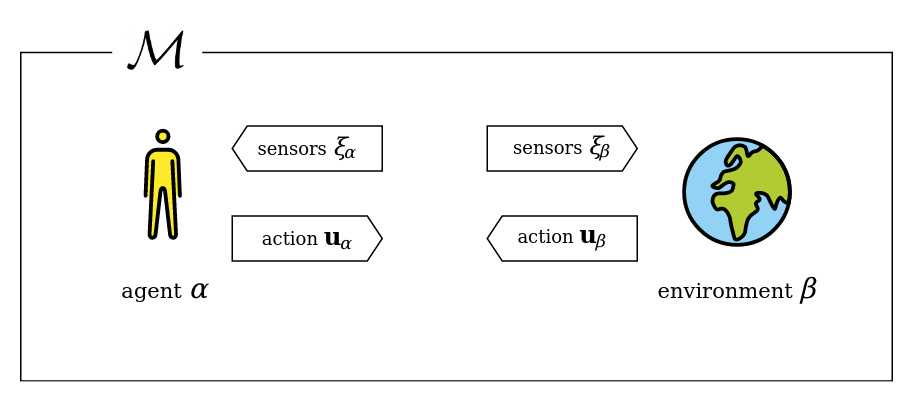
\includegraphics[width=12cm, keepaspectratio]{img/3_1_model.png.png}
	\caption{The model $\mathcal{M}$ and its components.}
\end{figure}

Let us define how this structure works.

Let $\mathcal{S}$ be the state space of dimension $m$, such that $\textbf{s} \in \mathcal{S}$ is a state of the model $\mathcal{M}$ and let $\mathcal{O}$ be the space of its observable states, having dimension $n$.
Both the \textit{agent} and the \textit{environment} can obtain full or partial information about the observable state $\textbf{o} \in \mathcal{O}$ through a series of \textit{sensors}.
We denote $\textbf{o}_\alpha \subseteq \textbf{o}$ the observable state sensed by the \textit{agent} and with $\textbf{o}_\beta \subseteq \textbf{o}$ the observable state sensed by the \textit{environment}.
Let $\xi_\alpha$ and $\xi_\beta$ be the two functions defined respectively as $\xi_\alpha: \mathcal{S} \to \mathcal{O}$ and $\xi_\beta: \mathcal{S} \to \mathcal{O}$ that, given a state $\textbf{s}$, return the observable state $\textbf{o}_\alpha$ and $\textbf{o}_\beta$.
$$ \xi_\alpha(\textbf{s}) = \textbf{o}_\alpha
\qquad \text{and} \qquad
\xi_\beta(\textbf{s}) = \textbf{o}_\beta $$

The distinction can be useful if we want to differentiate the level of the knowledge of the current state $\textbf{o}$ for $\alpha$ or $\beta$.
Such flexibility can be very useful to model specific cases of \textit{partial knowledge}.

Let $\mathcal{U}_\alpha$ be the space of dimension $l$ of all the possible actions of the \textit{agent} and let $\mathcal{U}_\beta$ be the space of dimension $r$ of all the possible actions of the \textit{environment}.
Let $\textbf{u}_\alpha \in \mathcal{U}_\alpha$ and $\textbf{u}_\beta \in \mathcal{U}_\beta$ be the actions taken.
Moreover, let $t$ be the time defined over the $\mathbb{R}$ space.
The simulator $f_\mathcal{M}$ (or simply $f$) that computes the evolution of our CPS, is defined as $f: \mathcal{S} \times \mathcal{U}_\alpha \times \mathcal{U}_\beta \times \mathbb{R} \to \mathcal{S}$ and, in particular, it is a differential equation of the form:
$$ \dot{s} = f(\textbf{s}, \textbf{u}_\alpha, \textbf{u}_\beta, t) $$

We can discretize it with respect to time $\Delta t = t_{i+1} - t_i$ and we obtain:
$$ \textbf{s}_{i+1} = \textbf{s}_i + f(\textbf{s}_i, (\textbf{u}_\alpha)_i, (\textbf{u}_\beta)_i, t_i) $$

where $i$ is the $i$-th discrete instant of time of the simulation.
We have now a discrete simulator that is able to compute the evolution of the CPS deterministically given the control actions.

Since the simulator is very dependent on the specific case study, in the next chapter we cover some examples of the equations used.

The simulator plays a crucial role: the NNs are not trained using observed examples.
Similarly to what happens in reinforcement learning \cite{reinforcementlearning}, we simply provide a simulated environment in which different choices can be made without real consequences.
This allows for a fast learning procedure that can encourage safe actions and penalize those that lead to undesired results.

In the next chapter, we describe in details how our \textit{case studies} are designed.

\subsection{Controller-Environment architecture}
The architecture is clearly inspired by that of a GAN.
In fact, we have two NNs that compete in a \textit{minimax} game for maximizing opposite goals.

The architecture is composed of:
\begin{itemize}
  \item the \textbf{attacker}, denoted by $A$, similar to a GAN \textit{generator},
  \item the \textbf{defender}, denoted by $D$, that tries to keep the CPS safe in the test scenarios.
\end{itemize}

The main difference compared to GANs is that there is no \textit{discriminator}.
The aim of the \textit{attacker} is to generate \textit{environment} configurations in which the \textit{defender} is not able to act safely, rather than trying to fool it.

Let us now describe the interaction between the physical model $\mathcal{M}$ and our adversarial NNs.
The \textit{defender} NN $D$ is the controller of the \textit{agent} in the model $\mathcal{M}$, while the \textit{attacker} is in charge of generating the worst possible configuration of the \textit{environment}.

The architecture of the two NNs can be whatever fits the problem at best.
Though, the power of the proposed approach is given by how the training is carried out, not by the NNs' design.

The two NNs produce a sequence of actions $\textbf{u}_\alpha$ and $\textbf{u}_\beta$.
Since in our approach there is no notion of time and only the state of our model $\mathcal{M}$ in a specific instant $t_i$ is known, we need our NNs to produce, for each timestep, a whole sequence of actions.
To make this possible we introduce the \textit{policy function} $\Pi_A$ for the \textit{attacker} NN e $\Pi_D$ for the \textit{defender} NN.

Let $\textbf{w}_A$ and $\textbf{w}_D$ be the coefficients' vectors defined on the spaces $\mathbb{R}^p$ and $\mathbb{R}^q$, respectively.
Let the notation $t_i \dots t_{i+h}$ denote a timeframe defined over $h$ instants.
From now on, this notation will denote sequences defined on the interval $[i, i+h]$.

The \textit{policy function} is a polynomial functions of the coefficients $\textbf{w}_i$ that produces as output a function $\textbf{u}(t)$ that, discretized as $\textbf{u}(t_i) = \textbf{u}_i $ for each timestep between $t_i$ and $t_{i+h}$, gives the sequence of actions $\textbf{u}_i \dots \textbf{u}_{i+h}$ for the considered horizon $h$.
In particular we define $\Pi_A: \mathbb{R}^p \times \mathbb{R} \to \mathcal{U}_\beta$ and $\Pi_D: \mathbb{R}^q \times \mathbb{R} \to \mathcal{U}_\alpha$ separately for each NN:
\begin{align*}
 \Pi_A(\textbf{w}_{Ai}, t)  = 
 \sum_j^p (\mathrm{w}_j)_{Ai} \cdot t^j = \textbf{u}_\beta(t)
& \quad \text{with}\quad
 \textbf{w}_{Ai} = A(\theta_A, \textbf{o}_{\beta i}, \textbf{z}_i) \\
 \Pi_D(\textbf{w}_{Di}, t)  = 
 \sum_j^q (\mathrm{w}_j)_{Di} \cdot t^j = \textbf{u}_\alpha(t)
& \quad \text{with}\quad
 \textbf{w}_{Di} = D(\theta_D, \textbf{o}_{\alpha i})
\end{align*}
The choice of the \textit{policy function} can be NN specific: for instance, they could use polynomials with different degree.

Using such \textit{policy function} has the advantage of introducing a natural smoothing and preventing an incoherent behaviour of the actions $\textbf{u}$ in two subsequent instants.

The problem of finding the best action $\textbf{u}$ has become the problem of finding the best coefficients $\textbf{w}_A$ and $\textbf{w}_D$ for the \textit{policy functions} $\Pi_A$ and $\Pi_D$.
And this is precisely the problem addressed by our NNs.
Despite the two NNs are very similar, we are going to cover them separately.

Let $\theta_A$ be the matrix of the weights and biases (the parameters) of the \textit{attacker} NN, defined on the space $\Theta_A$ of dimension dependent on NN's architecture.
As said before, the \textit{attacker} controls the \textit{environment}.
Therefore, at time $t_i$ it takes as input its own parameters $\theta_{Ai}$, the observable state $\textbf{o}_{\beta i}$ and a vector of \textit{gaussian} noise $\mathbf{z}_i \in \mathbb{R}^g$,  $\mathbf{z}_i  \sim \mathcal{N}(0, 1)$.
The introduction of such random input vector $\textbf{z}$ is borrowed from usual GANs literature: as we have seen in the previous chapter, it is possible to use this \textit{latent variable} to sample from the \textit{latent space}. 
The \textit{attacker} NN is defined as $A: \Theta_A \times \mathcal{O} \times \mathbb{R}^g \to \mathbb{R}^p$ and can be represented as the following function:
$$ A(\theta_A, \textbf{o}_{\beta i}, \textbf{z}_i) = \textbf{w}_{Ai}$$

The \textit{defender}, similarly to his opponent, controls the \textit{agent} and take as input its parameters $\theta_D$ -- the matrix of weights and biases defined over the space $\Theta_D$ of dimension dependent on NN's architecture -- and its observable state vector $\textbf{o}_{\alpha i}$.
No noise is passed as input to the \textit{defender} since there is no need to learn a distribution.
This NN must simply find the best possible set of coefficients $\textbf{w}_{Di}$.
The function is defined as $D: \Theta_D \times \mathcal{O} \to \mathbb{R}^q$ and can be represented as:
$$ D(\theta_D, \textbf{o}_{\alpha i}) =  \textbf{w}_{Di} $$

By doing so, starting from a given state of the system $\textbf{s}_i$ (from which we can observe $\textbf{o}_{\beta i}$ and $\textbf{o}_{\alpha i}$), we obtain the optimal coefficients $\textbf{w}_{Ai}$ and $\textbf{w}_{Di}$ and, by means of the \textit{policy functions}, we obtain the optimal sequence of actions $(\textbf{u}_\beta)_i \dots (\textbf{u}_\beta)_{i+h}$ and $(\textbf{u}_\alpha)_i \dots (\textbf{u}_\alpha)_{i+h}$ for the model $\mathcal{M}$ in the horizon $h$.

Given the sequences of actions in the time horizon $h$, we can now simulate via $f$ the complete evolution of the system $\mathcal{M}$.
The simulation is carried out step by step from time $t_i$ to $t_{i + h}$: at time $t_i$, a pair of actions $(\textbf{u}_\beta)_i$ and $(\textbf{u}_\alpha)_i$ is passed to $f$ that makes the system evolve into a state $\textbf{s}_{i+1}$ and so on.
Throughout the simulation we keep track of the sequence of system's states and we collect its evolution $\textbf{s}_i \dots \textbf{s}_{i + h}$.

Given the STL formula $\Phi$ for the requirement and keeping track of the sequence of the model's states $\textbf{s}_i \dots \textbf{s}_{i + h}$ evolved from the actions of both the \textit{attacker} and \textit{defender}, it is possible to compute the \textbf{robustness} of the trajectories via STL {quantitative semantics} (the function $R$ to compute the quantitative semantics has been introduced in the previous chapter):
$$ \rho_i = R(\Phi, \textbf{s}_i \dots \textbf{s}_{i + h}) $$

\begin{figure}[H]
	\centering
	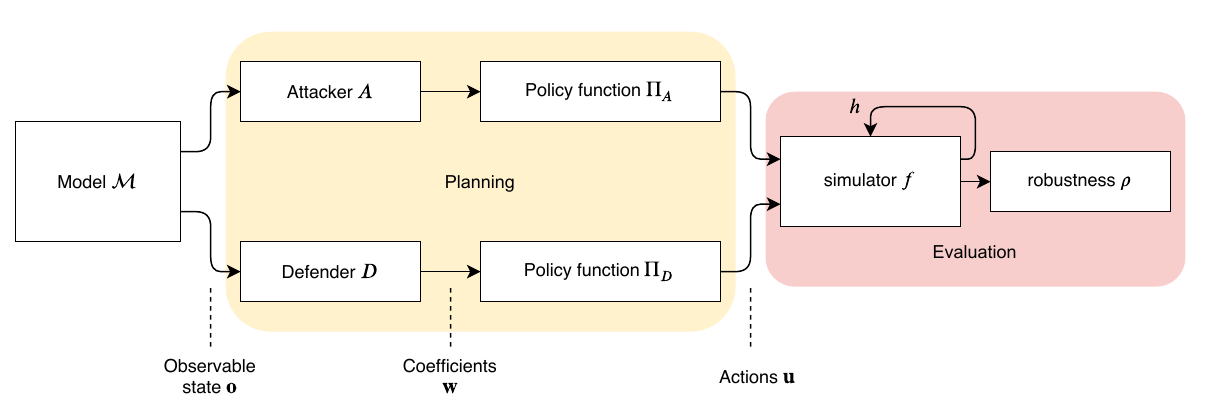
\includegraphics[width=14cm, keepaspectratio]{img/3_1_architecture.png}
	\caption{Diagram of the architecture. The model $\mathcal{M}$ observable state $\textbf{o}$ is the input of the two NNs that produce the coefficients $\textbf{w}$ for the policy functions $\Pi$. These functions gives the actions that are simulated for $h$ steps and the robustness of the system's evolution is computed.}
\end{figure}

The STL \textit{quantitative semantics}, as said in the previous chapter, measures the maximum shift that can be applied to a trajectory without varying the truth value of the requirements $\Phi$.
Therefore it is straightforward to use the \textit{robustness} $\rho$ as \textit{objective function} for tuning of the internal parameters of the NNs.

The \textit{robustness} is the quantity on which the two NNs play the \textit{minimax} game.
For convenience, let $F$ be a function $F: \mathcal{S} \times \Theta_D \times \Theta_A \to \mathcal{S}^h$ that, given a initial state $\textbf{s}_i$ of $\mathcal{M}$ and the parameters of the two NNs $\theta_D$ and $\theta_A$, computes the system's evolution in the horizon $h$:
$$ F(\textbf{s}_i, \theta_D, \theta_A) = \textbf{s}_i \dots \textbf{s}_{i+h} $$
Such function applies iteratively the simulator function $f(\textbf{s}_i, (\textbf{u}_\alpha)_i, (\textbf{u}_\beta)_i, t_i) = \textbf{s}_{i+1}$ for each pair of actions $(\textbf{u}_\alpha)_i = \Pi_D(D(\theta_D, \textbf{o}_{\alpha i}),t_i)$ and $(\textbf{u}_\beta)_i = \Pi_A(A(\theta_A, \textbf{o}_{\beta i}, \textbf{z}_i), t_i)$ computed in the interval $t_i \dots t_{i+h}$.
Then the \textit{loss function} is defined as follows:
$$ \mathscr{L}(\theta_A, \theta_D) = R(\Phi, F(\textbf{s}_i, \theta_D, \theta_A)) $$

Therefore, the \textit{minimax} game between the two is$$ \underset{\theta_A}{\min} \; \underset{\theta_D}{\max} \; \mathscr{L}(\theta_A, \theta_D) $$

In this setting, the \textit{defender} is going to tune its NN's weights in such a way to maximize the \textit{robustness} by generating safe actions for the model, while the \textit{attacker} is going to tune its NN's weights trying to generate more and more challenging scenarios for the opponent with the aim of minimizing its \textit{robustness}.


\section{Training}
The training approach borrows from the \textit{reinforcement learning} literature \cite{reinforcementlearning}.
The training is expressed as a sequence of \textbf{episodes} in which our \textit{agent} receives a feedback -- the \textit{robustness} -- for its choices and learns from it.

We define an \textit{episode} as a single safety problem to be solved.
At the beginning of each \textit{episode}, a new state $\textbf{s}_0$ of the model $\mathcal{M}$ is generated randomly to allow both the\textit{attacker} and the \textit{defender} to explore and learn from different configurations of the setting.
Then, each of them plans a strategy for the time horizon $h$, the whole evolution is simulated through $F$, and the \textit{robustness} of the specific sequence of choices is then computed in order to optimize the weights of the NNs.

Since the NNs do not take into account the past history of the opponents' actions and base the predictions solely on the current state $\textbf{s}_i$, it is possible to imagine each instant of the evolution of the system as a separate problem to solve.
This specific property that does not make any assumption on the system's evolution, allows to deal with problems using a simple architecture.
However, to explore reasonably well all the state space $\mathcal{S}$, it requires a specific kind of training in order to avoid undefined behaviours due to completely unexplored scenarios.

Due to this architecture's characteristic, in fact, it is compulsory to sample from the entire state space $\mathcal{S}$ in order to expose the NNs even to the less probable cases.
The \textit{hyper-grid} -- on which all the possible states lie -- is explored randomly adding some noise drawn from a normal distribution $\mathcal{N}(\mu, \sigma)$ where $\mu$ and $\sigma$ are respectively the mean and the variance specified according to the case study in order to maximize the diversity of the samples even in case of repeatedly sampled states.

For every sample drawn from the state space $\mathcal{S}$, a training \textit{episode} for a specific NN takes place.
The training, in fact, happens in a turn-based scheme where, both NNs make a choice but only one of them learns from that \textit{episode}.

For instance, suppose we are training $D$ at time $t_0$ and suppose we sample a state $\textbf{s}_0$, the parameters $\theta_A$ of the other NN remain constant for the specific \textit{episode}.
The following operations take place for each \textit{episode}:
\begin{align*}
 \Pi_A(A(\overline{\theta_A}, \xi_\beta(\textbf{s}_0), \textbf{z}_0), t) & = \textbf{u}_\beta(t) \\
 \Pi_D(D(\theta_D,  \xi_\alpha(\textbf{s}_0)), t) & = \textbf{u}_\alpha(t) \\
F(\textbf{s}_i, \theta_D, \overline{\theta_A}) & = \textbf{s}_0 \dots \textbf{s}_h \\
R(\Phi,  \textbf{s}_0 \dots \textbf{s}_h) & = \rho
\end{align*}
At this stage, the \textit{robustness} value $\rho$ is used only to compute the \textit{loss function} of $D$ and, hence, the backpropagation of the gradient affects only the internal parameters of the \textit{defender}.
The training of $A$ is conducted in the very same fashion.

Each training \textit{episode} can be repeated multiple times in order to make the NN try new alternative moves in the same scenario.
This strategy encourages the \textit{exploration} of different possible outcomes.
In particular, it is possible to make each NN repeat the \textit{episodes} a variable number of times.
Such mechanism is borrowed from classical GANs and it is used to balance the game between the two NNs: sometimes the task of one NN is much simpler than the other's, therefore, it needs to be artificially balanced.
Setting a different number of repetition for each NN, hence, increases the chances of convergence and prevents a NN from outperforming the other not allowing it to learn at all. 

\begin{algorithm}[H]
\setstretch{1}
\caption{Training procedure}
\begin{algorithmic}[1]
\Procedure{TrainStep}{}
    \State $s_0 \gets$ SampleRandomState()
    \For{attacker\_repetitions} \Comment{Train $A$}
        \State $z \gets \mathcal{N}(0,1)$
        \State $w_\beta \gets A(\theta_A, \xi_\beta(s_0), z)$
        \State $w_\alpha \gets D(\theta_D, \xi_\alpha(s_0))$
        \\
        \State states := [\:]
        \State states[$0$] $\gets s_0$
        \For{$i \gets 0 \dots h-1$}
            \State $u_{\alpha i} \gets \Pi_D(w_\alpha, i)$
            \State $u_{\beta i} \gets \Pi_A(w_\beta, i)$
            \State states[$i+1$] $ \gets f(s_i, u_{\alpha i}, u_{\beta i}, t_i)$
        \EndFor
        \\
        \State $\rho \gets R(\Phi, \text{states})$ 
        \State BackPropagation($A, \rho$)
        \State UpdateWeights($A$)
    \EndFor
    \\
    \State $s_0 \gets$ SampleRandomState()
    \For{defender\_repetitions} \Comment{Train $D$}
        \State $z \gets \mathcal{N}(0,1)$
        \State $w_\beta \gets A(\theta_A, \xi_\beta(s_0), z)$
        \State $w_\alpha \gets D(\theta_D, \xi_\alpha(s_0))$
        \\
        \State states := [\:]
        \State states[$0$] $\gets s_0$
        \For{$i \gets 0 \dots h-1$}
            \State $u_{\alpha i} \gets \Pi_D(w_\alpha, i)$
            \State $u_{\beta i} \gets \Pi_A(w_\beta, i)$
            \State states[$i+1$] $ \gets f(s_i, u_{\alpha i}, u_{\beta i}, t_i)$
        \EndFor
        \\
        \State $\rho \gets R(\Phi, \text{states})$ 
        \State BackPropagation($D, \rho$)
        \State UpdateWeights($D$)
    \EndFor
\EndProcedure
\end{algorithmic}
\end{algorithm}


\section{Testing}
Once a sufficiently high number of \textit{episodes} has been completed, the two NNs are ready to be used as \textit{controller} and {test generator} of our CPS.
It is possible to use the two NNs separately: in fact, once trained, they become completely independent one from the other.

The testing phase differs slightly from the training one since, in real scenarios, we do not have \textit{episodes} but a continuous evolution of the system.
Therefore, the strategy of computing an optimal plan for the time horizon $h$ and applying it, does not fit such scenario.

We took inspiration from the \textit{Model Predictive Control} algorithm \cite{mpc} to design the application of our method: in simple words, at each timestep $t_i$, the optimal strategy over $h$ steps is computed as in the training step but, instead of passing all the actions $\textbf{u}_i \dots \textbf{u}_{i + h}$ to the simulator, we execute only the first one and, on the next iteration, the new state $\textbf{s}_{i + 1}$ is used to compute the next move.
More precisely, the following operations are repeated iteratively:
\begin{align*}
 \Pi_A(A(\overline{\theta_A}, \xi_\beta(\textbf{s}_i), \textbf{z}_i), t) & = \textbf{u}_\beta(t) \\
 \Pi_D(D(\overline{\theta_D},  \xi_\alpha(\textbf{s}_i)), t) & = \textbf{u}_\alpha(t) \\
 f(\textbf{s}_i, (\textbf{u}_\alpha)_i, (\textbf{u}_\beta)_i, t_i) & = \textbf{s}_{i + 1}
\end{align*}

Since the NNs are trained and they are not learning anymore, we marked both their parameters with an overline.

Due to the iterative scheme of the policies, the proposed method acts as a \textbf{closed-loop} CPS.
At timestep $t_i$, in fact, an action is taken with respect to the time horizon $h$ and the new state $\textbf{s}_{i+1}$ is reached.
Through the \textit{sensors}, our NNs will be able to retrieve the observed state $\textbf{o}_{i+1}$ that will be used to compute the next action.
Such iterative procedure allows to handle automatically cases in which the desired state is not fully reached due to unexpected causes: the algorithm will plan a new optimal strategy starting from the new observed states, hence taking into account the possible errors that have been made.

\begin{algorithm}[H]
\setstretch{1}
\caption{Test procedure}
\begin{algorithmic}[1]
\Procedure{Execute}{$\mathcal{M}$, timesteps}
    \For{$i \gets 0 \dots$ timesteps}
        \State $s_0 \gets$ GetState($\mathcal{M}$)
        \\
        \State $z \gets \mathcal{N}(0,1)$
        \State $w_\beta \gets A(\theta_A, \xi_\beta(s_0), z)$
        \State $w_\alpha \gets D(\theta_D, \xi_\alpha(s_0))$
        \\
        \State $u_\beta \gets \Pi_A(w_\beta, 0)$
        \State $u_\alpha \gets \Pi_D(w_\alpha, 0)$
        \\
        \State DoAction($\mathcal{M}, u_\alpha, u_\beta$)
    \EndFor
\EndProcedure
\end{algorithmic}
\end{algorithm}
